\documentclass[12pt]{article}
\usepackage{times}
\usepackage[english]{babel}
\usepackage[utf8x]{inputenc}
\usepackage[colorinlistoftodos]{todonotes}
\usepackage[margin=1in]{geometry}
\usepackage{graphicx}
\usepackage{epstopdf}
\usepackage{cite}
\usepackage{listings}
\usepackage{dtklogos}
\usepackage{wrapfig}
\usepackage{subfigure}
\usepackage{amsmath}
\usepackage{amsthm}
\usepackage{amssymb}
\usepackage{amscd}
\usepackage{caption}
\usepackage{etoolbox}
\usepackage{fancyhdr}
\usepackage{stackengine}
\usepackage[export]{adjustbox}
\usepackage{url}
\patchcmd{\thebibliography}{\section*{\refname}}{}{}{}
\usepackage[document]{ragged2e}    %This causes text to left align
\usepackage[colorlinks=true, linkcolor=black,citecolor=black,urlcolor=blue]{hyperref}
\bibliographystyle{IEEEtran}
\DeclareGraphicsRule{.tif}{png}{.png}{`convert #1 `dirname #1`/`basename #1 .tif`.png}

\title{MCHE 220: Report 1}

\begin{document}
\lefthyphenmin3
\righthyphenmin4
% \pretolerance=2000
% \tolerance=500 
% \emergencystretch=10pt
%\raggedright     %Stops LaTeX from automatically hyphenating the right margin to fit better
%Combine this with \usepackage[document]{ragged2e} to get a text align left similar to natural MS Word
%-------------------------------------------------------------
%Header
%-------------------------------------------------------------
\fancyhf{}  
  \renewcommand{\headrulewidth}{0pt}
  \fancypagestyle{plain}{
    \fancyhead[R]{\thepage}} 
    \pagestyle{plain}
    
\captionsetup[table]{labelsep=space}

\begin{flushleft}
\hrulefill\\\hrule height 1pt
\vspace{5pt}
\textbf{DATE: }\today
\bigskip\\
\textbf{TO: }Sally Anne McInerny, Ph.D.\\ Department of Mechanical Engineering
\bigskip\\
\textbf{FROM: }Matthew J. Begneaud
\bigskip\\
\textbf{COPY: }John Guillory, Ph.D.\\ Department of Mechanical Engineering
\bigskip\\
\textbf{SUBJECT:} Electrical Resistance of an Aqueous Soluble Salt Solution
\vspace{-10pt}
\end{flushleft}
\hrulefill \hrule height 1pt

%-------------------------------------------------------------
%Start of Paper
%-------------------------------------------------------------

\section*{\fontsize{12}{12}\selectfont INTRODUCTION}
This memorandum conveys the findings of an experiment conducted to observe the effects that depth and separation distance of electrodes have on the resistance of a fluid solution. The objectives of this experiment are to:

\begin{itemize}

\item Measure the electrical current in an aqueous soluble salt solution caused by two cylindrical electrodes, positioning the electrodes at various combinations of depth and separation distance
\item Use Ohm's Law to calculate the resistance at each recorded configuration using the current recorded
\item Develop a regression model to predict the resistance of the solution at given configurations

\end{itemize}


The resistance should somewhat closely resemble that of a solid in terms of parameter effects. As such, it is expected that the regression should be somewhat similar to that of solids \cite{physics_book}, seen in Equation (1) where $\rho$ is density, $L$ is length of the solid, and $A$ is the cross-sectional area normal to which the electrical current travels. It is expected, for the fluid solution, that an increased distance will increase the resistance since there is more material between the electrodes, and that an increase in electrode depth will lower the resistance since there is effectively more cross-sectional area which allows the electric current to travel with more ease. The regression model proposed for the system is shown by Equation (2), where $S$ is separation distance, $d$ is depth, $R_o$ is the resting-state resistance of the system without the solution present. In accordance with the preceding statements, it is expected that the exponent $b1$ will be negative.
\bigskip

\begin{equation}
R = \rho\frac{L}{A}
\end{equation}

\begin{equation}
R-R_o = ad^{b_1}S^{b_2}
\end{equation}


\newpage

\begin{figure}[t!] %  figure placement: here, top, bottom, or page
   \centering
   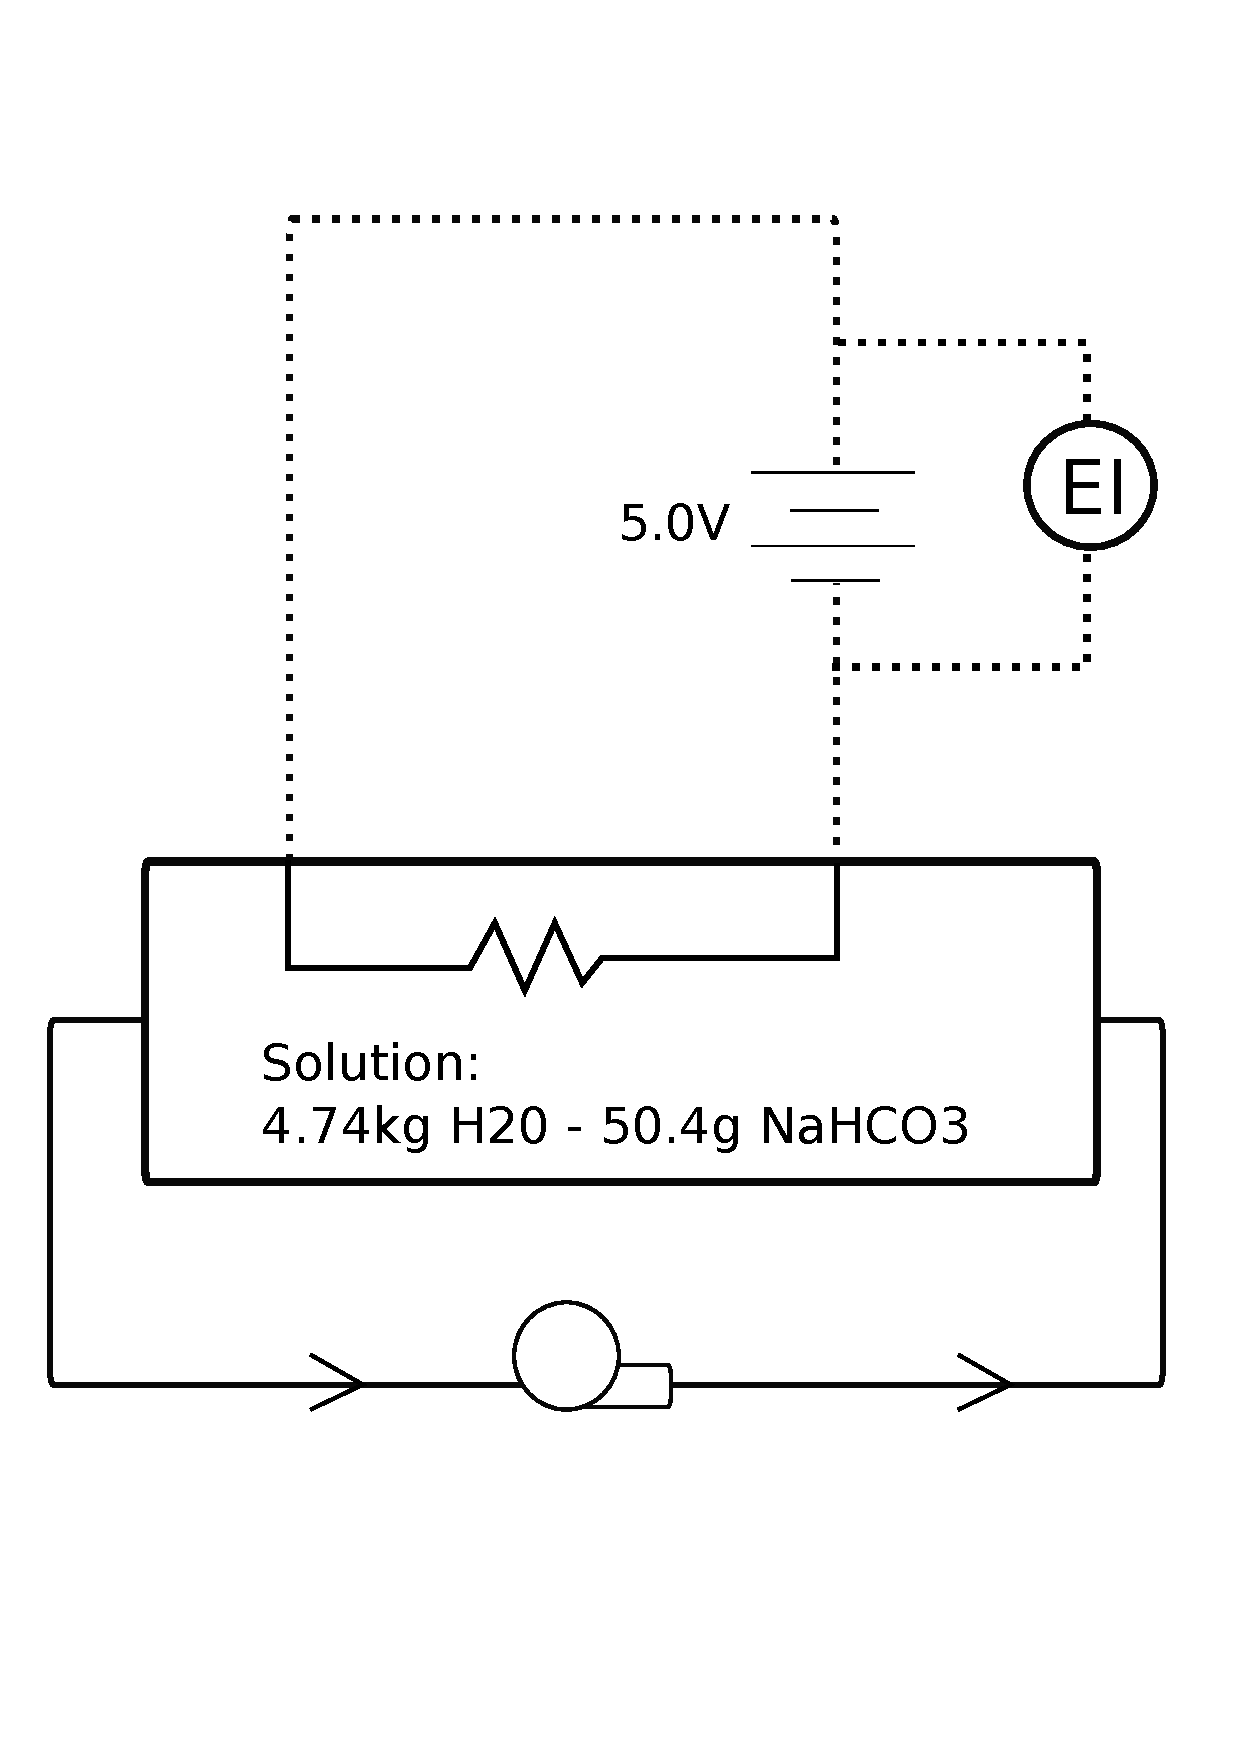
\includegraphics[width=4in]{system_diagram.pdf} 
   \caption{Experiment System Diagram}
   \label{fig:example}
\end{figure}

\section*{\fontsize{12}{12}\selectfont PROCEDURE}
The experiment system diagram is shown in Figure 1. The system consists of a voltage source, two cylindrical electrodes, a fish-tank pump, and the $H_2O - NaHCO_3$ solution itself. A Latin-Squares matrix is chosen to build a database which equally represents the effects of both parameters on the resistance. In this experiment, the electrode depth parameter is measured from the surface of the solution to the bottom of the electrode, and the separation parameter is the center-to-center distance between the two cylindrical electrodes. 
\bigskip

As shown in Figure 1, an electric current is induced in the solution via the electrodes and is recorded by observation of a current indicator device. A fish-tank pump is used to maintain a consistent flow of the solution which keeps the resistance uniform throughout the experiment. The recorded current is then used along with the recorded excitation voltage to calculate the equivalent resistance of the system.


\section*{\fontsize{12}{12}\selectfont DATA PRESENTATION \& ANALYSIS}
The data recorded during the experiment can be seen in Appendix A1. The calculated resistance data is also depicted in Figure 2 as a function of depth and separation distance, with depth on the abscissa and separation distance as a chosen parameter. Using Microsoft Excel, the coefficients for the model proposed in Equation (2) have been calculated, shown in Equation (3). The regression model has been superimposed on the data plot in Figure 2 for the minimum, maximum, and one intermediate level of electrode separation.
\bigskip

\begin{equation}
R-R_o = 105.5\frac{S^{0.25}}{d^{0.77}}
\end{equation}

\bigskip

The correlation coefficient calculated for the model is $r_{xy}=0.9905$. The f-statistic calculated is $f=233.35$, corresponding to a probability $P_r << 0.1\%.$




\begin{figure}[t!] %  figure placement: here, top, bottom, or page
   \centering
   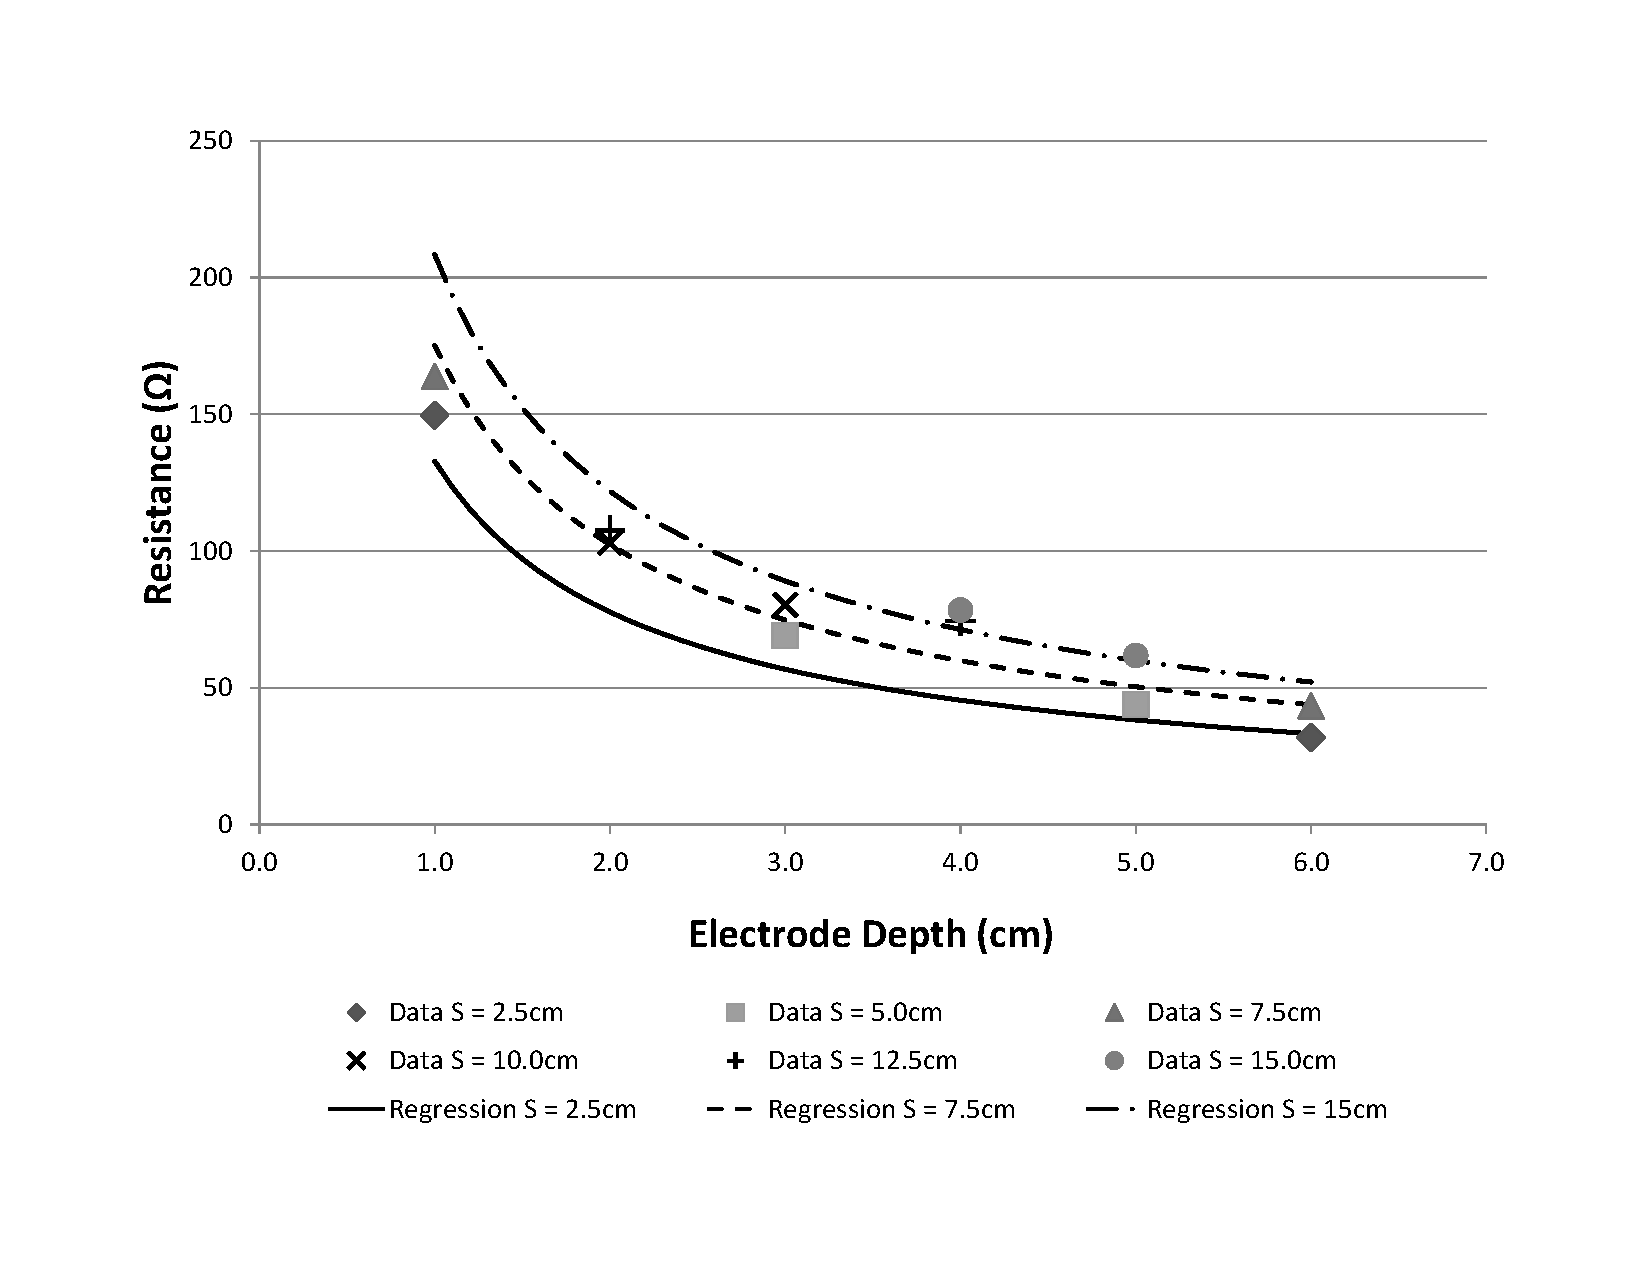
\includegraphics[width=\linewidth]{data_and_regression.pdf} 
   \caption{Resistance Data \& Regression Model}
   \label{fig:example}
\end{figure}

\section*{\fontsize{12}{12}\selectfont DISCUSSION}
It can be seen graphically in Figure 2 that the regression matches the data well. The correlation coefficient, calculated to be $r_{xy}=0.9905$, gives confidence that the regression model is sufficiently accurate. The calculated f-statistic, $f=233.35$, implies that the $P_r$ is much less than 0.1\%, meaning that there is a very low chance that either of the independent variables analyzed carries no relationship with the resistance of the system. In other words, the chances of the Null Hypothesis being true is almost zero, so the system can be considered to be well represented by the model with respect to the two parameters analyzed.
\bigskip

It can be seen from Figure 2 that the resistance increases as the electrode separation distance increases, which is similar to the effect of length on the resistance through a solid medium. The depth of the electrodes is seen to be inversely proportional to the resistance, which is similar to the effect of increased cross-sectional area on the resistance in a solid medium. This is because an increased electrode depth is analogous to adding more cross-sectional area between the two electrodes. In the preceding statements, it is clear that is an accurate assumption that the model for the resistance in the fluid would be similar to that of the resistance through a solid.

\section*{\fontsize{12}{12}\selectfont CONCLUSION}

\begin{itemize}

\item It has been shown that the resistance of the aqueous soluble salt solution can be modeled by similar means as for a solid material, depending largely on the distance the current must travel through the medium as well as the cross-sectional area through which it must travel.

\item The proposed regression model accurately depicts the behavior of the system analyzed in this experiment, as seen in Figure 2 and by the calculated correlation coefficient $r_{xy}=0.9905$.

\item There is virtually no chance as indicated by the calculated f-statistic $f=233.35$ that the Null Hypothesis is true for the proposed model, as the probability that it is true is much less than 0.1\%

\end{itemize}



\section*{\fontsize{12}{12}\selectfont REFERENCES}

\begin{thebibliography}{2}

\bibitem{physics_book}
Halliday, D., Resnick, R., and Walker J., 2008, \emph{Fundamentals of Physics}, $8^{th}$ ed. Extended, John Wiley \& Sons, Inc., Hoboken, NJ, Chap. 26.

\end{thebibliography}




\newpage


\section*{\fontsize{14}{14}\selectfont APPENDIX}

\hrulefill

\section*{\fontsize{12}{12}\selectfont A1}

\begin{table}[h!]
\centering
\caption{Experiment Data}
\label{my-label}
\begin{tabular}{lll}
diameter (cm) & separation (cm) & current (mA) \\
\hline
1             & 2.5             & 33.4         \\
1             & 7.5             & 30.5         \\
2             & 10              & 48.5         \\
2             & 12.5            & 46.5         \\
3             & 5               & 72.3         \\
3             & 10              & 62.2         \\
4             & 12.5            & 67.2         \\
4             & 15              & 63.7         \\
5             & 5               & 114          \\
5             & 15              & 80.9         \\
6             & 2.5             & 157.2        \\
6             & 7.5             & 115.4       
\end{tabular}
\end{table}



\end{document}
----------------------------%TEmplates-------------------------------

-------------------------Figure-----------------------

\begin{figure}[h!]  
  \centering
    \includegraphics[width=\linewidth]{**file**}
    \caption{Docking Station}
\end{figure}

---------------------------Table-----------------------
\begin{table}[ht]
\caption{Nonlinear Model Results} % title of Table
\centering % used for centering table
\begin{tabular}{c c c c} % centered columns (4 columns)
\hline\hline %inserts double horizontal lines
Case & Method\#1 & Method\#2 & Method\#3 \\ [0.5ex] % inserts table
%heading
\hline % inserts single horizontal line
1 & 50 & 837 & 970 \\ % inserting body of the table
2 & 47 & 877 & 230 \\
3 & 31 & 25 & 415 \\
4 & 35 & 144 & 2356 \\
5 & 45 & 300 & 556 \\ [1ex] % [1ex] adds vertical space
\hline %inserts single line
\end{tabular}
\label{table:nonlin} % is used to refer this table in the text
\end{table}



probably best to insert as an image from excel

\bigskip\\
\begin{table}[h!]
  \caption{}
  \includegraphics[width=\linewidth]{**file**}
\end{table}
\bigskip\\





-----------------------------Equations------------------------
-----------------------------Regular
\begin{equation}
a = b + c
\end{equation}

--------------------------------- Multiline
\begin{multline}
a = b + c + d + e + f
+ g + h + i + j \\
+ k + l + m + n + o
\end{multline}

-------------------------------Citations-------------------------
\bibitem{Author last name}
  Last, First., year of publication,
  article name, book(etc) name, from \\
  link goes here

----------------------------------other-----------------------------

equations:
http://moser-isi.ethz.ch/docs/typeset_equations.pdf

citations:
http://library.missouri.edu/engineering/about/guides/asme
https://www.asme.org/shop/proceedings/conference-publications/references